

\section{Experiments - Installations}
The workings of a Transformer and the workings of Generative Pre-Training 2 Transformer are described in Section \ref{transformer-intro}. While it is proposed there that they are similar, in the experiments they are totally separate.

There are several basic neural network models. One is the basic sequence-to-sequence GRU model typically used for neural machine translation. There are also two Transformers and the Generative Pre-Training 2.  

There are only three Raspberry Pi boards and a Jetson Nano board used here. Three Raspberry Pi installations were successful. The Nano is used for an additional GPT2 installation, serving as a speed comparison with the Raspberry Pi. 


\subsection{Questions}
This list of questions was asked of all models. 

\begin{verbatim}
Hello.
What is your name? 
What time is it?
What do you do?
What is your favorite color?
Do you like red?
Do you like blue?
What is your favorite candy?
Do you like ice cream?
Good bye.
\end{verbatim}

Without considering reply time, the GPT2 model worked best. 

Subjectively, the first Transformer model with the Persona corpus did not perform as well as the Generative Pre-Training 2 model. It did not perform better than the Gated Recurrent Unit model either. 

The model from the GRU tutorial performed well. It was better than the initial Transformer model and on par with the larger Transformer model. It was not better than the GPT2.

\subsection{Checklist} 

This checklist is visited and revisited to subjectively rate the chatbots.

\begin{itemize}
	
	\item [1.] Are all the responses in plain English? Are any of the answers gibberish?
	
	\item [2.] Is there a  variety of answers? Are all answers the same?
	
	\item [3.] Does the model give good answers to the questions about `favorite color' and `favorite candy?' The model could have a set of easy answers that it can use for this kind of question or it considers the question separately. 
	
	\item [4.] `No' is a safe answer for many types of question as it is clearly English, it follows logically, and it is short and easy to remember. Another safe answer is `I don't know.' Does the model use these answers at all times?
	
	\item [5.] Does the model answer well to `Hello' and `Good bye?'
	
\end{itemize}

The reasons for questions 1, 2 and 5 are straight forward. The reason for question 3 is to determine how well the model understands English. If the answers to `favorite candy' and `favorite color' are the same, then the model is simple. If the answers are different, then the answer set the model uses is larger. The model might or might not know there is a difference between candy and color. 

A simpler model will answer `I don't know' for the `favorite candy' and `favorite color' questions. It can even answer questions like `do you like red' and `do you like ice cream' with `I don't know.' 

For question 4, simple `No' answers are used frequently to answer questions that would otherwise need complex sentence structure. A simpler model learns during training that `No' answers are easier to remember and could be applied in many places.

\section{Chatbot - Gated Recurrent Unit Model}
There is a model based on the sequence-to-sequence architecture proposed by Vinyals et al \cite{DBLP:journals/corr/VinyalsL15}.
%This first model, largely written by hand, does not work very well. 
It is from an online tutorial by  Inkawhich et al \cite{2018Inkawhich} trained on a large English corpus. 

This model does not use a Transformer architecture. It answered a number of subjective questions appropriately. 

\label{chatbot-gru-tutorial-used}

\subsection{Questions}
This screen shot is the sample question list as it was answered by the GRU model.

%\begin{minipage}{2in}
\begin{verbatim}
> hello .
you re a good man .
> what is your name ?
smith .
> what time is it ?
i don t know .
> what do you do ?
i m a comedian .
> what is your favorite color ?
i don t know .
> do you like red ?
no .
> do you like blue ?
no .
> what is your favorite candy ?
it s a big one .
> do you like ice cream ?
no .
> good bye .
good bye .
\end{verbatim}
%\end{minipage}
%\bigskip


%\noindent \textbf{Checklist:} 
\subsection{Checklist}

\begin{itemize}
	\item [1.] \textbf{Are all the responses in plain English? Are any of the answers gibberish?}
	
	\item [] All the responses are in plain English. There is no gibberish.
	
	\item [2.] \textbf{Is there a  variety of answers? Are all answers the same?}
	
	\item [] Not all answers are the same.
	\item [3.] \textbf{Does the model give good answers to the questions about `favorite color' and `favorite candy?' The model could have a set of easy answers that it can use for this kind of question or it considers the question separately.} 
	
	\item[] It is debatable whether the answers to the questions about `favorite color' and `favorite candy' are good. It is good that the two types of questions don't have the same answers.
	
	\item [4.] \textbf{`No' is a safe answer for many types of question as it is clearly English, it follows logically, and it is short and easy to remember. Another safe answer is `I don't know.' Does the model use these answers at all times?}
	
	\item[] This model uses that answer at times. It does not use `no' always.
	
	\item [5.] \textbf{Does the model answer well to `Hello' and `Good bye?'}
	
	\item []The model answers well to `Hello' and `Good bye.'
\end{itemize}

This is a reasonably good and light weight model. The memory it uses is small and it replies quickly.

\section{Smart Speaker - Gated Recurrent Unit Model}

The GRU model was installed on a Raspberry Pi 3B, allowing tests of speech-to-text and text-to-speech libraries. The RAM requirements were less than 500MB and the trained model answered questions almost instantaneously. It was outfitted with a microphone and a speaker. It was also configured to run automatically on startup. For this experiment, the Pytorch library was compiled.

The model requires access to the Internet for the exchange that the speech-to-text software has to make with the Google servers.

As there was no monitor and it took some time for the model to launch, the program was coded to beep when the model was ready to accept input for the first time.

\section{Chatbot - Transformer Model with Persona Corpus}
\label{transformer-persona-corpus}
Using the Persona Corpus a Transformer model was trained, but not pre-trained. It did not use transfer learning. %The Persona Corpus comes from Mazar{\'{e}} et al \cite{DBLP:journals/corr/abs-1809-01984}.

This Transformer model uses the Tensorflow library, not Pytorch. Small, it uses 2 layers, 4 heads, a hidden size of 128, and has encoder and decoder sections.

The memory footprint, running below one Gigabyte, could be installed on a Raspberry Pi board. %That requires a python package called `tensorflow-model-server' and this package had to be provided for ARMv7 for the Raspberry Pi. 


\subsection{Questions}
Subjectively this Transformer model is not better than the original GRU from the sequence-to-sequence tutorial. It can respond to four or five sentences. The default reply sentence for unknown prompts is `Hi, how are you today?' It has answers to prompts like `hi,' `How are you?' and `What do you do?' It doesn't answer arbitrary questions. It cannot answer 'What is your favorite color?' It can not tell you the time. 

This is the sample question list as it was answered by the model.

\begin{verbatim}
> hello
hi , how are you today ?
> what is your name?
hi , how are you today ?
> what time is it ?
I like to read a lot
> what do you do ?
i'm a student
> what is your favorite color ?
hi , how are you today ?
> do you like red ?
hi , how are you today ?
> do you like blue ?
hi , how are you today ?
> what is your favorite candy ?
hi , how are you today ?
> do you like ice cream ?
yes , i do 
> good bye
hi , how are you today ?
\end{verbatim}

%\noindent \textbf{Checklist:} 
\subsection{Checklist}

\begin{itemize}
	\item [1.] \textbf{Are all the responses in plain English? Are any of the answers gibberish?}
	
	\item []All the responses are in plain English. There is no gibberish.
	
	\item [2.] \textbf{Is there a  variety of answers? Are all answers the same?}
	
	\item []There is a variety of answers. There is not a great variety though, and this is a problem for this model.
	
	\item [3.] \textbf{Does the model give good answers to the questions about `favorite color' and `favorite candy?' The model could have a set of easy answers that it can use for this kind of question or it considers the question separately.} 
	
	\item []Some of the answers are re-used and do not follow logically from the questions. The `favorite color' and `favorite candy' questions prompt the model's default answer `Hi, how are you today?' 
	
	\item [4.] \textbf{`No' is a safe answer for many types of question as it is clearly English, it follows logically, and it is short and easy to remember. Another safe answer is `I don't know.' Does the model use these answers at all times?}
	
	\item []The model does not use `No' or `I don't know.'
	
	\item [5.] \textbf{Does the model answer well to `Hello' and `Good bye?'}
	
	\item []The model has an answer for `Hello' but not for `Good bye.'
	
\end{itemize}

This is a poor model. It does use English language answers, but does not perform well in many other respects.

\section{Smart Speaker - Transformer Model with Persona Corpus}

This Transformer model was tested on the Raspberry Pi 4B. 

The Transformer model takes two minutes to boot on the Raspberry Pi, the response time is slow, and the time between the first two or three responses is uncomfortably slow. After those first responses the time between answers gets to be more natural.

Though smart speaker installation was attempted and ultimately successful, the Raspberry Pi that was used was required for another model that worked better. % and was retained for the thesis.

\section{Chatbot - Transformer Model with Movie Corpus}

\label{transformer-movie-corpus}
A Transformer model was trained to use as a chatbot using the Movie Corpus. It was not pre-trained with any large corpus, and did not use transfer learning. 

This is the model referred to as the larger Transformer model. It is larger than the Transformer model with the Persona Corpus but it is smaller than the smallest GPT2 model.

This model uses the Tensorflow library, not Pytorch. 

The Persona corpus model uses 2 layers, 4 heads, and a hidden size of 128. In contrast, the Movie corpus model uses 6 layers, 8 heads, and a hidden size of 512, and has both encoder and decoder sections.

While running, the memory footprint of the Movie Corpus model was above 1.5 Gigabytes. The model was installed on a Raspberry Pi 4B board, requiring a Python package called `Tensorflow-model-server' which had to be built from source or otherwise provided for the Raspberry Pi. 

The model took seven days to train on the development computer in a x86\_64 environment with a CPU based processor. The goal for training was 50,000 lines of text. After training the loss graph was consulted and the installed version was culled from the saved checkpoint at the 45,000 line point.


\begin{figure}[H]
	\begin{center}
		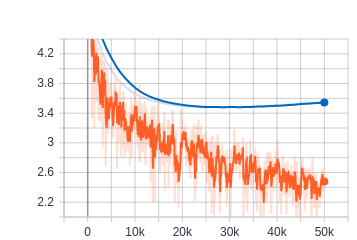
\includegraphics[scale=3.5]{Figure_2}
		
		
	\end{center}
	\caption[Loss - Larger Transformer Model]{Loss - Orange is training loss and blue is evaluation loss.}
	
	%\addcontentsline{lof}{section}{Word Embeddings}
\end{figure}

Subjectively this Transformer model is better than the one based on the smaller hyper-parameter set and the Persona Corpus.


%\begin{lstlisting}[language=bash]
\subsection{Questions}
This is the sample question list as it was answered by the model.

\begin{verbatim}
> Hello.
hello 
> What is your name?
i don't know 
> What time is it?
i don't know 
> What do you do?
what do you mean ?
> What is your favorite color?
i don't know 
> Do you like red?
no 
> Do you like blue?
yeah 
> What is your favorite candy?
i don't know 
> Do you like ice cream?
yeah 
> Good bye.
bye 
\end{verbatim}

%\noindent \textbf{Checklist:} 
\subsection{Checklist}

\begin{itemize}
	\item [1.] \textbf{Are all the responses in plain English? Are any of the answers gibberish?}
	
	\item []All the responses are in plain English. 
	
	\item [2.] \textbf{Is there a  variety of answers? Are all answers the same?}
	
	\item []There is a variety of answers. 
	
	\item [3.] \textbf{Does the model give good answers to the questions about `favorite color' and `favorite candy?' The model could have a set of easy answers that it can use for this kind of question or it considers the question separately. }
	
	\item []The `favorite color' and `favorite candy' questions are sometimes ignored. The model does not always have original answers for these questions. It will reply with `I don't know.' much of the time. This model does answer better than the model in Section \ref{transformer-persona-corpus}.
	
	\item [4.] \textbf{`No' is a safe answer for many types of question as it is clearly English, it follows logically, and it is short and easy to remember. Another safe answer is `I don't know.' Does the model use these answer at all times?}
	
	\item []The model does in fact use `No' or `I don't know.' It does not use these exclusively.
	
	\item [5.] \textbf{Does the model answer well to `Hello' and `Good bye?'}
	
	\item []The model does have an answer for `Hello' and `Good bye.'
\end{itemize}

This is a reasonably good model and it is preferable to the model that uses the Persona Corpus.

\section{Smart Speaker - Transformer Model with Movie Corpus}

The Transformer model is installed on the Raspberry Pi. It takes two minutes to boot and 6 seconds to answer any question. 

The Raspberry Pi gives a tone at the end of loading the model to signal the model is finished. % processing input. % during long response times. 
%This tone notifies the user that the model is loaded and ready to respond to questions. 
%The model is also configured to beep intermittently during operation to signal that it is processing an input. 
This is helpful for a configuration where there is no monitor.

A set of LED lights is installed on the Raspberry Pi to show when the model is processing input and when the model can take new input. %The lights are helpful.


\section{Chatbot - Generative Pre-Training 2 Model}

\label{install-gpt2-chatbot}
A pre-trained GPT2 model with the large English corpus, called `WebText,' was used to produce a chatbot.% to ascertain if the model works better than the sequence-to-sequence model. 
%In our tests this worked well and this model was considered superior. 
This model was not trained in the typical sense after download. 

Though the large 774M model was available, the smaller 117M model was used in this test on the Raspberry Pi. It was later tested on the Jetson Nano.

For these experiments, the GPT2 was used in `zero-shot' mode. This means there was no special fine-tuning of the model in the application.

Special coding for the input and output was required to operate it as a chatbot. 

Output was limited to about 25 tokens. Input to the model was prepended with the character string `Q:' by our code. Output was observed to have the character string `A:' prepended to it. It is assumed therefore that the model was at some point exposed to the `Question/Answer' paradigm in written passages during its training. %This was helpful.

Output from the model was usually larger in size than needed. Also, output had the character of having some sensible utterance followed by some output that was only a partial sentence.

It was necessary to process the output. 
%First, it was checked for the "A:" character string at the beginning. If it was there it was removed. 
If the `A:' character string was found at the beginning it was removed.
Then the first complete sentence was used as output, while words and phrases after that were discarded.

\subsection{Context Experiment}
The model was given details that it could draw on during normal execution. 
There were two choices. One choice, train the model using fine-tuning and transfer-learning to recognize certain questions and to supply answers. The other choice showed the model a list of relevant facts before every input sequence. This information would be summarized with each reply.

The second choice was preferred. The text that the model was shown always included the name of the model (picked arbitrarily) along with information about the location, occupation, and time. When the model is shown the time, it is always the latest system time.

Occasionally the model would report the wrong time. %This sort of activity is mysterious.

\subsection{GPT2 Fact Sheet}

The GPT2 chatbot is shown a paragraph or table with each question. The table below shows the contents of the paragraph. 

%There is not enough room with the other models, like the Transformer or the GRU model, to include this kind of a fact sheet or fact paragraph. 

Subject matter like that found in the `favorite color' question and the `favorite candy' question are not found in the table.

\begin{table}[h]
	\begin{center}	
		
		\begin{tabular}{lll}
			Num & Question             & Answer                        \\
			\hline \hline
			1   & What is your name?   & My name is Jane.              \\
			2   & What time is it?     & It is 12:00, January 1, 2020. \\
			3   & What do you do?      & I am a student.               \\
			4   & Where are you?       & I am in New York.             \\
			5   & How are you feeling? & I am happy.                  \\
			\hline     
		\end{tabular}
	\end{center}
	\label{fig-fact-sheet}
	\addcontentsline{lot}{section}{GPT2 Fact Overview}
	
\end{table}


\subsection{History Experiment}
From each question all input and output was concatenated and included with the next question. The goal was for the model to treat the `Q' and `A' as historical input and then refer to that information as it answered new questions. This didn't always work as expected. At times the model was confused by the extra input and at others there was no effect. 

Without this mechanism the model has no notion of temporal context. The answers to questions could not depend on the answers to past questions. %Though this historical input did not always work, the code is retained in the hopes that at some point it is useful.

Consider the questions below.
\begin{verbatim}
> Do you like the color red?
I like the color red.
> What is your favorite color?
Red.
\end{verbatim}

\label{install-gpt2-history}

%We like this output. 
The model is asked about the color `red.' Doing so the model is encouraged to pick `red' as the answer to the next question about color. When `favorite color' is requested, `red' is the answer. Without any history the model will answer the `favorite color' question with another answer. It may answer `pink' or it may answer `the colors of the rainbow.' 

From one sentence to the next the model is keeping track of the context of the conversation. History is considered. However it is not always the case that the model chooses the color recently discussed as the `favorite' color.


\subsection{Program Launching}

Programming that allowed the model to launch programs when directed by the user was implemented. In this way the project moved closer to commercially produced smart-speakers. The code used string manipulation and simple keyword recognition rather than the model's neural-network. This code can be enabled when the model is run from the command line, but not for the Raspberry Pi as it runs headless.

There is no memory prohibition for using the program launching code on the Raspberry Pi. Future work may use Chromecast to connect the Raspberry Pi with the user's home TV or monitor. 

\subsection{Summary}

Subjectively this model was the best of those tested. Usually the model would answer questions about it's location, it's name, and the time, correctly. %Interestingly there where times when it did not do so. 
Incorrect answers did address the particular question asked. Sometimes it used alternative answers. For example, it would answer with a time but not the correct time or a city but not the correct city.  %This was odd.

The output was always sensible English. 
 
Any subject matter could be chosen and the model would answer. The prompts did not need to be the same as the simple introductory conversation of the Transformer model. 

\subsection{Questions}
This is the sample question list as it was answered by the model. Note that the information mentioned in the answer about the time was accurate when the test was run.

\begin{verbatim}
> hello
Hello.
> what is your name ?
My name is Jane.
> what time is it ?
02:59 PM January 28, 2020.
> what do you do ?
I am a student.
> what is your favorite color ?
I love the color of the rainbow.
> do you like red ?
Yes.
> do you like blue ?
I do.
> what is your favorite candy ?
I love candy.
> do you like ice cream ?
I do. 
> good bye
Good bye.
\end{verbatim}

%\noindent \textbf{Checklist:} 
\subsection{Checklist}

\begin{itemize}
	\item [1.] \textbf{Are all the responses in plain English? Are any of the answers gibberish?}
	
	\item []All the responses are in plain English. 
	
	\item [2.] \textbf{Is there a  variety of answers? Are all answers the same?}
	
	\item []There is a variety of answers. 
	
	\item [3.] \textbf{Does the model give good answers to the questions about `favorite color' and `favorite candy?' The model could have a set of easy answers that it can use for this kind of question or it considers the question separately. }
	
	\item []The answers to the questions about `favorite color' and `favorite candy' are good and better than many other models. However, the model could have a set of answers that it can use for this kind of question. The model seems to know what candy is and that a color is something different. The answers are good but not perfect.
	
	\item [4.] \textbf{`No' is a safe answer for many types of question as it is clearly English, it follows logically, and it is short and easy to remember. Another safe answer is `I don't know.' Does the model use these answer at all times?}
	
	\item []The model does not use `I don't know' often. 
	
	\item [5.] \textbf{Does the model answer well to `Hello' and `Good bye?'}
	
	\item []The model does have an answer for `Hello' and `Good bye.'
	
\end{itemize}

The model will answer with it's name and you can tell it your name, but it is confused by the latter. It will on occasion tell you that it's name and your name are the same. This is in part because it cannot remember what it most recently said to you or what you most recently said to it. 

It's also in part because it cannot always distinguish between the `Q:' and `A:' prompts.

This is the best model tested, but it is relatively large and that aspect makes it difficult to apply in some cases.

\section{Smart Speaker - Generative Pre-Training 2 Model}

\label{install-gpt2-smart}
Code was added that uses text-to-speech and speech-to-text libraries, so that the model could respond to auditory cues and commands.

The model was installed on two small computers, the Raspberry Pi and the Jetson Nano.% The Nano is discussed in Section \ref{chapter-nano}.

The model was installed on the Raspberry Pi 4B with 4GB of RAM. The Pytorch Python library for ARMv7 was compiled for this model. 
While execution on the production laptop was instantaneous, execution on the Raspberry Pi took 13 to 15 seconds for every response. (See the discussion of `Reply Time' in Section \ref{setup-reply-time}.)

The program was modified to sound a tone during processing. Without this it would have been difficult to know when to speak. Also LED lights were installed to indicate when the model is processing input and when the model can take new input. %The lights are helpful.
